\section{CAPÍTULO III: LOS DATOS}\label{sec:los-datos}

\subsection{Tipos de Variables}\label{sec:tiposdevariables}

Dentro de las 47 variables descriptivas a utilizar antes mencionadas también se incluyen 4 variables que muestran la evolución temporal por intervalos de los pacientes. Estas variables son:

\begin{itemize}
    \item Flujo de Oxígeno
    \item Frecuencia Respiratoria (FR)
    \item Escala SAPI (Sistemas de Alerta Precoz Infantil)
    \item Score Wood-Downes
\end{itemize}

Estas 4 variables no han sido tratadas como series temporales dada la baja frecuencia de recolección durante las primeras 24 h de ingreso; que es el intervalo temporal al que ha sido acotado el estudio. Las tres primeras (Flujo de Oxígeno, Frecuencia Respiratoria y Escala SAPI)variables han sido recopiladas 3 veces durante las primeras 24h del ingreso del paciente pediátrico y la última (Score Wood-Downes) ha sido recogida a la llegada del paciente y a las 24 h. Es decir estas variables describen la estancia del paciente en intervalos.  Estas variables serán catalogadas como \textit{Temporales en Intervalos.} 

Si tratamos estas 3 últimas variables como temporales nos quedarían solamente 36 variables descriptivas. (3 variables temporales $\times$ 3 intervalos + 1 $\times$ 2 intervalos = 11 variables) y por otro lado 2 variables en forma de series temporales. Cada variable de estas contiene 1441 datos. (60 minutos $\times$ 24 horas + 1\textsuperscript{er} dato repetido
= 1441).

Dentro de las 36 variables descriptivas restantes se encuentran 3 variables que dan información más allá de las primeras 24 h de monitorización. Estas variables en principio serán excluidas del estudio y son:

\begin{itemize}
    \item Días con Gafas Nasales
    \item Días con O$_2$
    \item Días con OAF
\end{itemize}

Estas 3 variables serán catalogadas como: \textit{Descriptivas fuera del scope}. El \textit{scope} será básicamente las primeras 24 h de ingreso del paciente pediátrico.

Por último dentro de las 33 variables descriptivas dentro del \textit{scope} se encuentran 2 variables que no son ni cualitativas ni cuantitativas. Estas variables serán catalogadas como \textit{Otras}. Las 31 variables restantes serán catalogadas como \textit{Descriptivas dentro de scope}.

En la tabla \ref{tabla:variables_estudio} se muestran las diferentes variables recopiladas para realizar el presente estudio. 

\begin{table}[H]
    \centering
        \begin{tabular}{| m{5cm} | m{1.75cm} | m{7cm} |}
            \hline Tipo de Variable & Cantidad & Nombres  \\ \hline
            Descriptivas dentro de scope & 31 & Edad, Peso, Sexo, Edad Gestacional (EG), Palivizumab, Lactancia Materna (LM), Dermatitis, Alergias, Tabaco, Enfermedad Base, Radiografía, Analítica, Suero, Etiología, Prematuridad, Alimentación, Sonda Nasogástrica, Gafas Nasales al Ingreso, OAF, OAF al ingreso, OAF tras ingreso, Horas de Ingreso tras inicio OAF, UCIP, Deterioro, Pausas de Apnea, PCT (Procalcitonina en la sangre), PCR (Prueba de Proteína C relativa), Leucocitos, Nautrófilos, Linfocitos y Score Cruces Ingreso  \\ \hline
            Descriptivas fuera de scope & 3 & Días con Gafas Nasales, Días con O$_2$ y Días con OAF. \\ \hline
            Temporales en 3 Intervalos & 11 & Frecuencia Respiratoria (0 - 8 h), Frecuencia Respiratoria (8 - 16 h),
            Frecuencia Respiratoria (16 - 24 h),
            Flujo O$_2$ (0 - 8 h),
            Flujo O$_2$ (8 - 16 h),
            Flujo O$_2$ (16 - 24 h),
            SAPI (0 - 8 h),
            SAPI (8 - 16 h), 
            SAPI (16 - 24 h), Score Wood-Downes Ingreso y Score Wood-Downes 24 h . \\ \hline
            Series Temporales & 2 & Frecuencia Cardiaca, Saturación de Oxígeno \\ \hline
            Otras & 2 & Notas e Identificador Paciente. \\ \hline
        \end{tabular}
    \caption{Variables Usadas en el Estudio}\label{tabla:variables_estudio}
\end{table}

Las variables temporales han sido recopiladas durante las primeras 24 h del ingreso del paciente pediátrico cuando mostraba un cuadro bronquiolítico. La frecuencia con la que han sido recopilados los datos ha sido de 1 vez cada minuto. En la siguiente Figura \ref{fig:fc-JJB} se muestra un ejemplo de la evolución  variable \textit{Frecuencia Cardiaca} en forma de serie temporal y de la misma forma la Figura \ref{fig:satO2-JJB} pero para la \textit{Saturación de O$_2$}. Estas dos series temorales pertenecen a la evolución del paciente pediátrico \textit{JJB\_11182744}.

\begin{figure}[H]
    \centering
    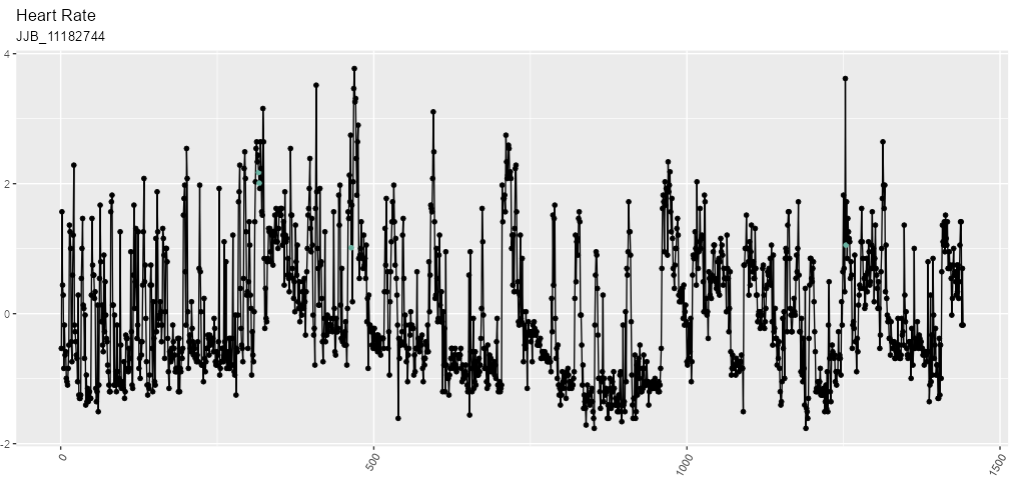
\includegraphics[scale=0.70]{./img/Heart-Rate-JJB.png}
    \caption{Valores de Frecuencia Cardíaca del paciente \textit{JJB\_11182744}}
    \label{fig:fc-JJB}
\end{figure}

\begin{figure}[H]
    \centering
    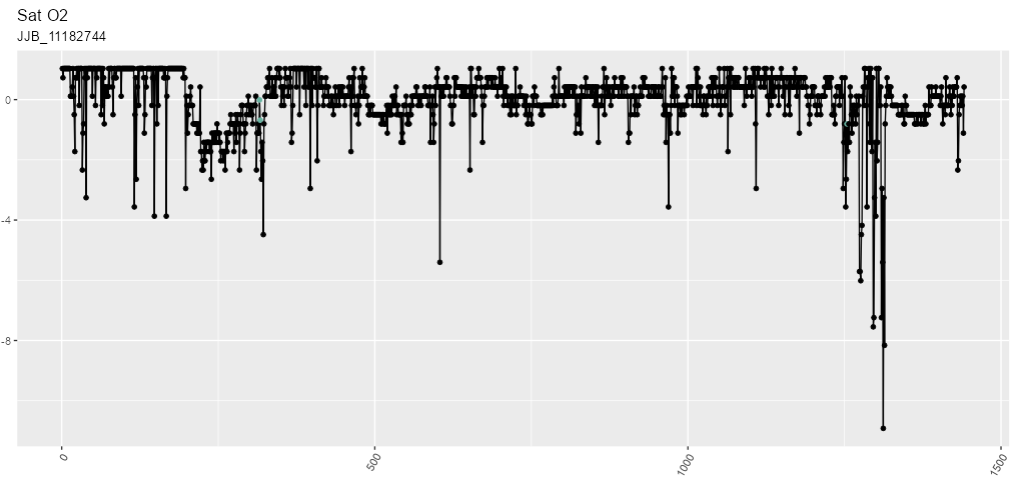
\includegraphics[scale=0.70]{./img/SatO2-JJB.png}
    \caption{Valores de Saturación de O$_2$ del paciente \textit{JJB\_11182744}}
    \label{fig:satO2-JJB}
\end{figure}

A la hora de trabajar con variables temporales se ha de tener en cuenta que los datos temporales pueden ser de dos tipos: \textit{Discretos} o \textit{Continuos}. Los datos discretos son aquellos que se recogen en intervalos de tiempo, por ejemplo, el número de pacientes que llegan a un hospital cada hora. Los datos continuos son aquellos que se recogen de forma continua, por ejemplo, en nuestro caso la saturación y frecuencia cardíaca de un paciente cada minuto.

Para terminar esta Sección \ref{sec:tiposdevariables} una última cuestión a valorar son las variables cualitativas y cuantitativas que se han recopilado. Las variables cualitativas son aquellas que describen una cualidad del paciente, por ejemplo, el sexo o la edad gestacional. Las variables cuantitativas son aquellas que describen una cantidad del paciente, por ejemplo, la frecuencia cardíaca o la saturación de oxígeno.

En la siguiente Tabla \ref{tabla:cuali_cuanti} se muestra la división entre variables cualitativas y cuantitivas recopiladas en el estudio y dentro del \textit{scope}.

\begin{table}[H]
    \centering
        \begin{tabular}{| m{5cm} | m{1.75cm} | m{7cm} |}
            \hline Tipo de Variable & Cantidad & Nombres  \\ \hline
            Cuantitativas & 15 & Edad, Peso, Edad Gestacional (EG), Horas de Ingreso tras inicio OAF, PCT (Procalcitonina en la sangre), PCR (Prueba de Proteína C relativa), Leucocitos, Nautrófilos, Linfocitos, Frecuencia Respiratoria (0 - 8 h), Frecuencia Respiratoria (8 - 16 h),
            Frecuencia Respiratoria (16 - 24 h),
            Flujo O$_2$ (0 - 8 h),
            Flujo O$_2$ (8 - 16 h),
            Flujo O$_2$ (16 - 24 h). \\ \hline
            Cualitativas & 27 & Sexo, Palivizumab, Lactancia Materna (LM), Dermatitis, Alergias, Tabaco, Enfermedad Base, Radiografía, Analítica, Suero, Etiología, Prematuridad, Alimentación, Sonda Nasogástrica, Gafas Nasales al Ingreso, OAF, OAF al ingreso, OAF tras ingreso, UCIP, Deterioro, Pausas de Apnea, Score Cruces Ingreso, SAPI (0 - 8 h),
            SAPI (8 - 16 h), 
            SAPI (16 - 24 h), Score Wood-Downes Ingreso y Score Wood-Downes 24 h. \\ \hline
            Otras & 2 & Notas e Identificador Paciente. \\ \hline
        \end{tabular}
    \caption{Variables Cualitativas y Cuantitativas Dentro del \textit{Scope}}\label{tabla:cuali_cuanti}
\end{table}

\subsection{Preprocesamiento de los Datos}

En este apartado se describirá el procesamiento de los datos realizado para el presente estudio.

\subsubsection{Limpieza de Datos}\label{sec:limpieza_datos}

En primer lugar se ha realizado una limpieza de datos. Esta limpieza de datos ha consistido en varios pasos: 

\begin{enumerate}
    \item \textbf{Validación de Archivos:} Contrastar que los diferentes archivos de datos no contienen datos duplicados o incoherencias.
    \item \textbf{Cálculo de Medias:} Calcular de manera automatizada las medias de \textit{Frecuencia Respiratoria} y \textit{Saturación de Oxígeno} cada hora. Estas medias han sido facilitadas en el Archivo de Datos de Pacientes pero por rigor se han vuelto a calcular para cada paciente. Ya que además que en la Carpeta de Datos de Monitorización se guardan los datos brutos con los que los médicos han calculado estas medias. Además de estas $2$ medias horarias, se han hecho dos trasformaciones en los datos de \textit{Frecuencia Cardiaca} que se explicarán más tarde. (\textit{Frecuencia Cardiaca Escalada} y \textit{Frecuencia Cardiaca por Cuantiles})
    \item \textbf{Datos Faltantes:} Determinar que pacientes y variables tienen un alto número de datos faltantes y eliminarlos del estudio.
    \item \textbf{Variables No Relevantes:} Eliminar variables que no aportan información relevante para el estudio.
\end{enumerate}

\paragraph{Validación de Archivos}

 
Por parte del hospital se han recopilado 2 archivos de datos diferentes. Estos archivos de datos son:

\begin{itemize}
    \item \textbf{Archivo de Datos de Pacientes:} Este archivo contiene información descriptiva de los pacientes pediátricos. En este archivo se encuentran las variables contenidas en la Tabla \ref{tabla:cuali_cuanti}. Este archivo contiene 47 variables y 79 pacientes.
    \item \textbf{Carpeta de Datos de Monitorización:} En esta carpeta se almacena un archivo por cada paciente. Cada archivo contiene información temporal de los pacientes pediátricos. En este archivo se encuentran las variables \textit{Series Temporales} en la Tabla \ref{tabla:variables_estudio}. Por cada archivo se tienen 2 variables temporales (Saturación de O$_2$ y Frecuencia Cardiaca), cada variable presenta 1441 datos por paciente.
\end{itemize}

La Carpeta de Datos de Monitorización contiene 79 archivos de datos y el Archivo de Datos de Pacientes contiene 79 pacientes. Por lo tanto, se ha de contrastar que los datos de los pacientes contenidos en el Archivo de Datos de Pacientes estén contenidos en la Carpeta de Datos de Monitorización o si existen pacientes duplicados.

La cabecera de la Carpeta de Datos de Monitorización es la siguiente:
\begin{figure}[H]
    \centering
    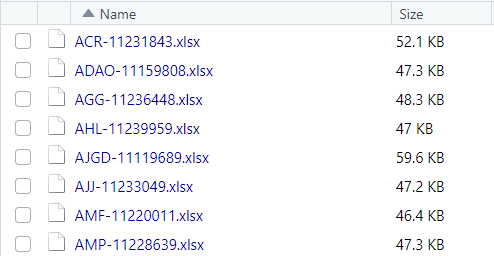
\includegraphics[scale=0.70]{./img/Carpeta-Monitor.png}
    \caption{Cabecera de la Carpeta de Datos de Monitorización}
    \label{fig:cabecera_monitorizacion}
\end{figure}

Y las primeras columnas del Archivo de Datos de Pacientes son las siguientes:
\begin{figure}[H]
    \centering
    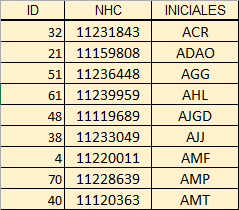
\includegraphics[scale=1.0]{./img/Archivo-Monitor.png}
    \caption{Cabecera de la Carpeta de Datos de Monitorización}
    \label{fig:cabecera_monitorizacion}
\end{figure}

Este contraste se ha automatizado de manera que para futuros estudios se pueda realizar de manera rápida y eficiente. El resultado de este contraste ha sido que los datos de los pacientes contenidos en el Archivo de Datos de Pacientes están contenidos en la Carpeta de Datos de Monitorización. Existían algunas desviaciones en los nombres pero fuero corregidas. Por lo tanto, no existen pacientes duplicados y se puede continuar con el estudio.

\paragraph{Cálculo de Medias}

En el Archivo de Datos de Pacientes venían calculadas las medias de \textit{Frecuencia Respiratoria} y \textit{Flujo de Oxígeno} cada hora. Estas medias han sido re-calculadas de manera automatizada para cada paciente y se han añadido al Archivo de Datos de Pacientes. Además de estas 2 medias se han hecho dos trasformaciones en los datos de \textit{Frecuencia Cardiaca} que se explicarán más tarde y se han calculado sus respectivas medias por hora. 

Se han calculado dos tipos de medias: 

\begin{itemize}
    \item \textbf{Medias No Nulas:} Se han calculado las medias de aquellos intervalos de hora dentro de las 24 h que no presentaban valores faltantes.
    \item \textbf{Medias Nulas:} Se han calculado las medias de aquellos intervalos de hora dentro de las 24 h sin importar si había momentos de valores valores faltantes dentro del intervalo hora.
\end{itemize}

Estos valores se han calculado para todos los pacientes, como modo de ejemplo el resultado para el paciente \textit{JJB\_11182744} ha sido el siguiente mostrado en la Tabla \ref{tabla:medias-JJB}:

% Se comienza una página nueva sin formato (sin número de página y sin encabezado/pie de página):
\newpage
\thispagestyle{empty}

% Se modifica la geometría (los márgenes) de la página y se coloca en formato horizontal:
\newgeometry{top=10mm, bottom=10mm, left=12mm, right=12mm}
\begin{landscape}

    \begin{table}[!ht]
        \centering
        \begin{tabular}{|l|l|l|l|l|l|l|l|l|l|l|l|}
        \hline
            hour & n & Missing\_FC & Missing\_SO2 & Mean\_FC & Mean\_SO2 & Mean\_Q & Mean\_SC & Mean\_FC\_NA & Mean\_SO2\_NA & Mean\_Q\_NA & Mean\_SC\_NA \\ \hline
            18 & 43 & 0 & 0 & 140,4186047 & 98,23255814 & 0,552067823 & -0,205230874 & 140,4186047 & 98,23255814 & 0,552067823 & -0,205230874 \\ \hline
            19 & 60 & 0 & 0 & 137,4666667 & 99,1 & 0,500688619 & -0,356544211 & 137,4666667 & 99,1 & 0,500688619 & -0,356544211 \\ \hline
            20 & 60 & 0 & 0 & 143,0166667 & 98,46666667 & 0,613802318 & -0,07205686 & 143,0166667 & 98,46666667 & 0,613802318 & -0,07205686 \\ \hline
            21 & 60 & 0 & 0 & 141,7 & 97,13333333 & 0,567600299 & -0,139547853 & 141,7 & 97,13333333 & 0,567600299 & -0,139547853 \\ \hline
            22 & 60 & 0 & 0 & 135,3666667 & 92,11666667 & 0,479248047 & -0,464188074 & 135,3666667 & 92,11666667 & 0,479248047 & -0,464188074 \\ \hline
            23 & 60 & 2 & 2 & ~ & ~ & ~ & ~ & 164,3448276 & 95,12068966 & 0,867006799 & 1,021202963 \\ \hline
            00 & 60 & 0 & 0 & 162,0666667 & 98,5 & 0,918496135 & 0,904426753 & 162,0666667 & 98,5 & 0,918496135 & 0,904426753 \\ \hline
            01 & 60 & 0 & 0 & 150,9833333 & 97,13333333 & 0,729509118 & 0,336306366 & 150,9833333 & 97,13333333 & 0,729509118 & 0,336306366 \\ \hline
            02 & 60 & 1 & 0 & ~ & 95,98333333 & ~ & ~ & 155,559322 & 95,98333333 & 0,762103523 & 0,570866889 \\ \hline
            03 & 60 & 0 & 0 & 142,3166667 & 96,01666667 & 0,606131522 & -0,107938147 & 142,3166667 & 96,01666667 & 0,606131522 & -0,107938147 \\ \hline
            04 & 60 & 0 & 0 & 142,2166667 & 96,86666667 & 0,569912026 & -0,113064045 & 142,2166667 & 96,86666667 & 0,569912026 & -0,113064045 \\ \hline
            05 & 60 & 0 & 0 & 130,6166667 & 97,8 & 0,37096502 & -0,70766824 & 130,6166667 & 97,8 & 0,37096502 & -0,70766824 \\ \hline
            06 & 60 & 0 & 0 & 155,8166667 & 96,4 & 0,762258703 & 0,584058113 & 155,8166667 & 96,4 & 0,762258703 & 0,584058113 \\ \hline
            07 & 60 & 0 & 0 & 132,55 & 96,73333333 & 0,405018753 & -0,608567541 & 132,55 & 96,73333333 & 0,405018753 & -0,608567541 \\ \hline
            08 & 60 & 0 & 0 & 129,4833333 & 97,06666667 & 0,344631214 & -0,765761753 & 129,4833333 & 97,06666667 & 0,344631214 & -0,765761753 \\ \hline
            09 & 60 & 0 & 0 & 127,8166667 & 97,18333333 & 0,312055141 & -0,85119339 & 127,8166667 & 97,18333333 & 0,312055141 & -0,85119339 \\ \hline
            10 & 60 & 0 & 0 & 151,2166667 & 96,43333333 & 0,703296936 & 0,348266795 & 151,2166667 & 96,43333333 & 0,703296936 & 0,348266795 \\ \hline
            11 & 60 & 0 & 0 & 156,55 & 97,41666667 & 0,87619425 & 0,621648034 & 156,55 & 97,41666667 & 0,87619425 & 0,621648034 \\ \hline
            12 & 60 & 0 & 0 & 145,95 & 98,1 & 0,685284072 & 0,078302822 & 145,95 & 98,1 & 0,685284072 & 0,078302822 \\ \hline
            13 & 60 & 0 & 0 & 146,4166667 & 98,13333333 & 0,704465169 & 0,10222368 & 146,4166667 & 98,13333333 & 0,704465169 & 0,10222368 \\ \hline
            14 & 60 & 0 & 0 & 129,9333333 & 97,08333333 & 0,372386073 & -0,742695211 & 129,9333333 & 97,08333333 & 0,372386073 & -0,742695211 \\ \hline
            15 & 60 & 1 & 1 & ~ & ~ & ~ & ~ & 155,220339 & 92,6779661 & 0,833584194 & 0,553490963 \\ \hline
            16 & 60 & 0 & 0 & 143,6333333 & 93,95 & 0,628285376 & -0,040447154 & 143,6333333 & 93,95 & 0,628285376 & -0,040447154 \\ \hline
            17 & 60 & 0 & 0 & 141,8666667 & 96,01666667 & 0,596238571 & -0,131004689 & 141,8666667 & 96,01666667 & 0,596238571 & -0,131004689 \\ \hline
            18\_1 & 18 & 0 & 0 & 156,1111111 & 96,05555556 & 0,890367072 & 0,599151036 & 156,1111111 & 96,05555556 & 0,890367072 & 0,599151036 \\ \hline
        \end{tabular}
        \caption{Medias Nulas y No Nulas de \textit{Frecuencia Cardíaca}, \textit{Saturación de O$_2$}, \textit{Cuantiles Cardíacos} y \textit{Frecuencia Cardíaca Escalada}  por hora para el paciente \textit{JJB\_11182744}}\label{tabla:medias-JJB}
    \end{table}

% Se devuelve el formato y la geometría de la página a sus valores originales:
\end{landscape}
\restoregeometry 

\paragraph{Datos Faltantes}

Se ha realizado un estudio de los datos faltantes. Este estudio ha consistido en determinar que pacientes y que variables tenían un alto número de datos faltantes y eliminarlos del estudio. 

\subparagraph*{Variables con Datos Faltantes} 

En la siguiente Figura~\ref{fig:missing-descriptive} se muestra la distribución de datos faltantes de las variables referenciadas en la Tabla \ref{tabla:cuali_cuanti}. 
 
\begin{figure}[H]
    \centering
    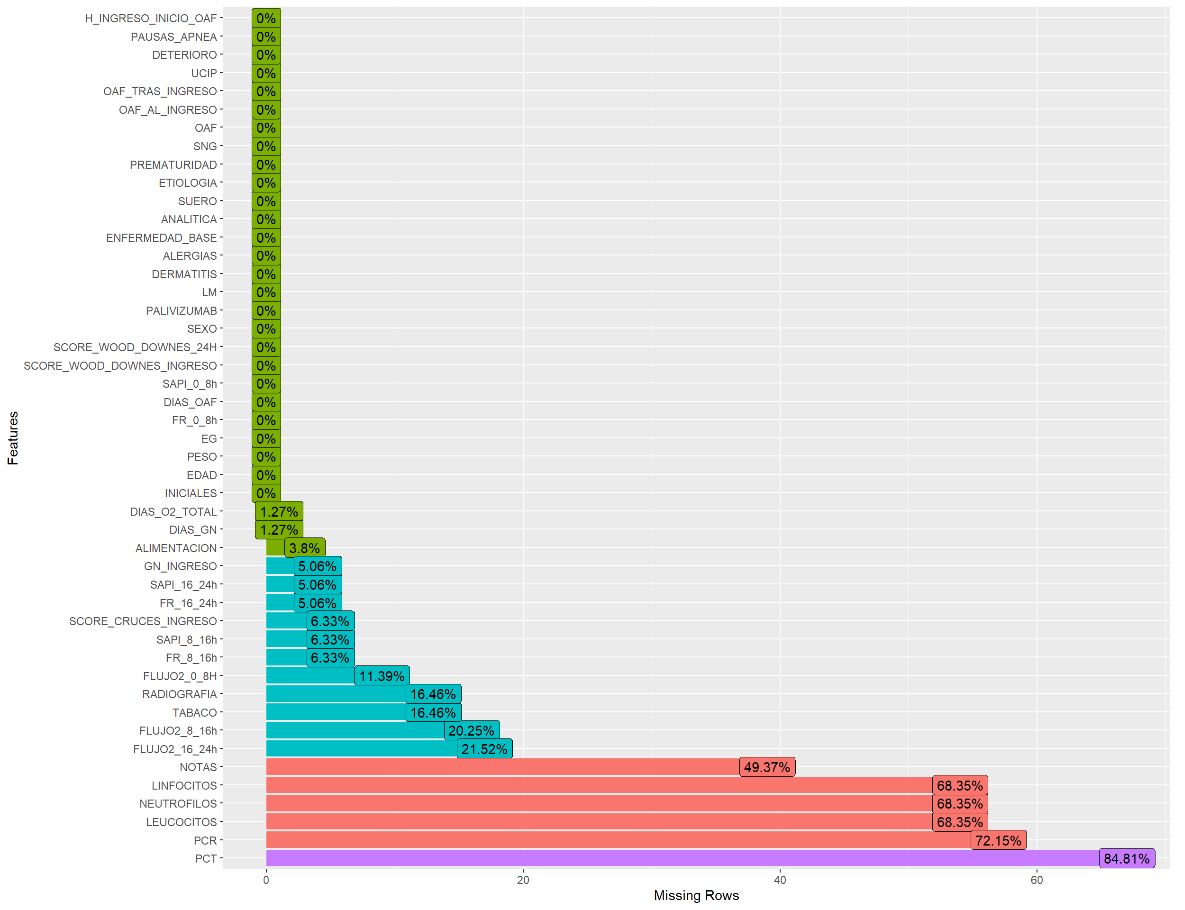
\includegraphics[scale = 0.70]{./img/missig-data-descriptive.png}
    \caption{Datos Faltantes en el Archivo de Datos de Pacientes}
    \label{fig:missing-descriptive}
\end{figure}

Por tro lado se ha estudiado que variables suelen faltar juntas. En la siguiente Imagen \ref{fig:missing-descriptive-cross} se muestra la distribución de datos faltantes cruzados de las 6 variables con mayor número de datos faltantes de la anterior Figura \ref{fig:missing-descriptive}.

\begin{figure}[H]
    \centering
    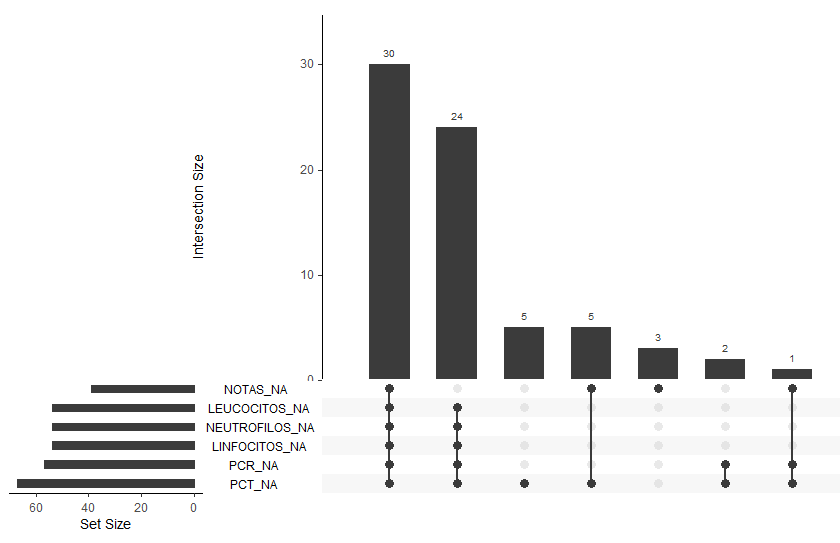
\includegraphics[scale = 0.70]{./img/missig-data-descriptive-cross.png}
    \caption{Datos Faltantes Cruzados de las 6 variables con Mayor Porcentaje de Datos Faltantes en el Archivo de Datos de Pacientes}
    \label{fig:missing-descriptive-cross}
\end{figure}

Según la Figura \ref{fig:missing-descriptive-cross} los \textit{Neutrofilos}, \textit{Linfocitos} y \textit{Leucocitos} se muestran faltantes siempre juntos, si falta uno faltan todos. Esto tiene sentido ya que los tres se obtienen si al paciente se le ha realizado una analítica. Por el contrario si solo contamos con los pacientes a los que se les ha realizado una analítica no hay faltantes de estas tres variables como se puede ver en la Figura \ref{fig:missing-descriptive-cross-analitica}. Es decir de manera sencilla, los datos faltantes de estas tres variables se deben a que no se le ha realizado una analítica al paciente.

\begin{figure}[H]
    \centering
    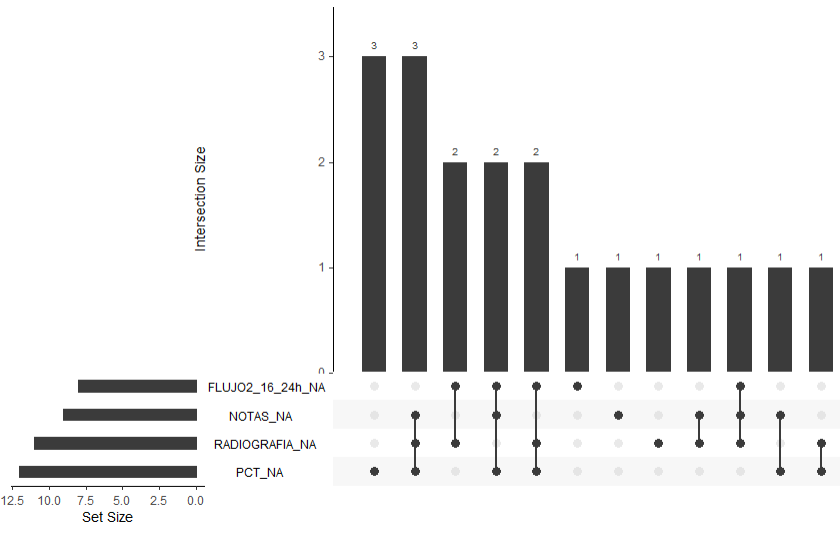
\includegraphics[scale = 0.70]{./img/missig-data-descriptive-cross-anal.png}
    \caption{Datos Faltantes Cruzados de las 4 variables con Mayor Porcentaje de Datos Faltantes en el Archivo de Datos de Pacientes si se le Ha Realizado una Analítica al Paciente}
    \label{fig:missing-descriptive-cross-analitica}
\end{figure}
\newpage


\subparagraph*{Pacientes con Datos Faltantes} 

Cuando se habla de pacientes con datos faltantes se hace referencia a aquellos pacientes que tienen datos faltantes en las variables \textit{Series Temporales} de la Tabla \ref{tabla:variables_estudio}. 

A cada paciente se le monitoriza durante las primeras 24 horas de su ingreso. En algunos casos, pueden ocurrir eventos que interrumpan la monitorización continua. Por ejemplo, si un paciente es trasladado a la Unidad de Cuidados Intensivos Pediátricos (UCIP), si es necesario realizarle alguna prueba o llevar a cabo tareas de higiene personal, se le desconecta de la monitorización. 

En la Figuras \ref{fig:fc-HGSDA} y \ref{fig:satO2-HGSDA} se muestran las \textit{Series Temporales} de \textit{Frecuencia Cardiaca} y \textit{Saturación de O$_2$} de el paciente \textit{HGSDA\_11233118} respectivamente. En estas se pueden observar como en ciertos momentos la monitorización se pausa y se registran valores faltantes en ciertos intervalos. 
\begin{figure}[H]
    \centering
    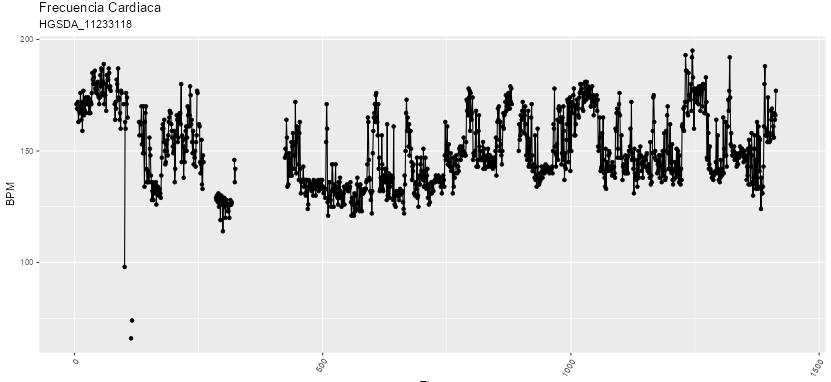
\includegraphics[scale=0.85]{./img/Heart-Rate-HGSDA.png}
    \caption{Valores de Frecuencia Cardíaca del paciente \textit{HGSDA\_11233118}}
    \label{fig:fc-HGSDA}
\end{figure}

\begin{figure}[H]
    \centering
    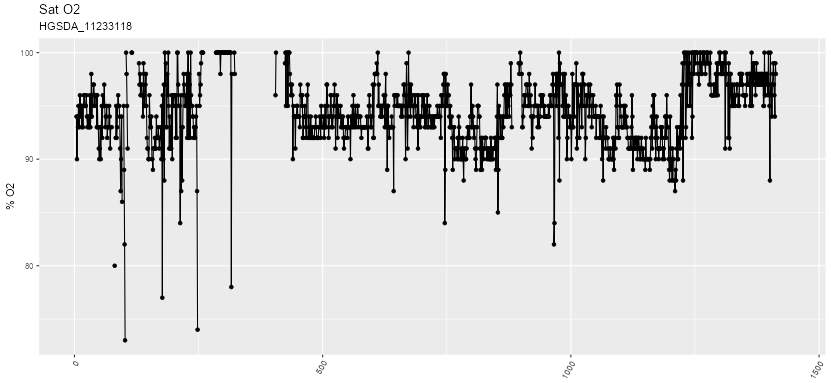
\includegraphics[scale=0.85]{./img/SatO2-HGSDA.png}
    \caption{Valores de Saturación de O$_2$ del paciente \textit{HGSDA\_11233118}}
    \label{fig:satO2-HGSDA}
\end{figure}


En la siguientes Figuras \ref{fig:missing-FC} y \ref{fig:missing-SatO2} se muestra la distribución y porcentaje de datos faltantes en las \textit{Series Temporales} de los 79 pacientes estudiados. La primera imagen hace referencia a la \textit{Frecuencia Cardiaca} y la segunda a la \textit{Saturación de O$_2$}.

% Se comienza una página nueva sin formato (sin número de página y sin encabezado/pie de página):
\newpage
\thispagestyle{empty}

% Se modifica la geometría (los márgenes) de la página y se coloca en formato horizontal:
\newgeometry{top=10mm, bottom=10mm, left=12mm, right=12mm}
\begin{landscape}

    \begin{figure}[H]
        \centering
        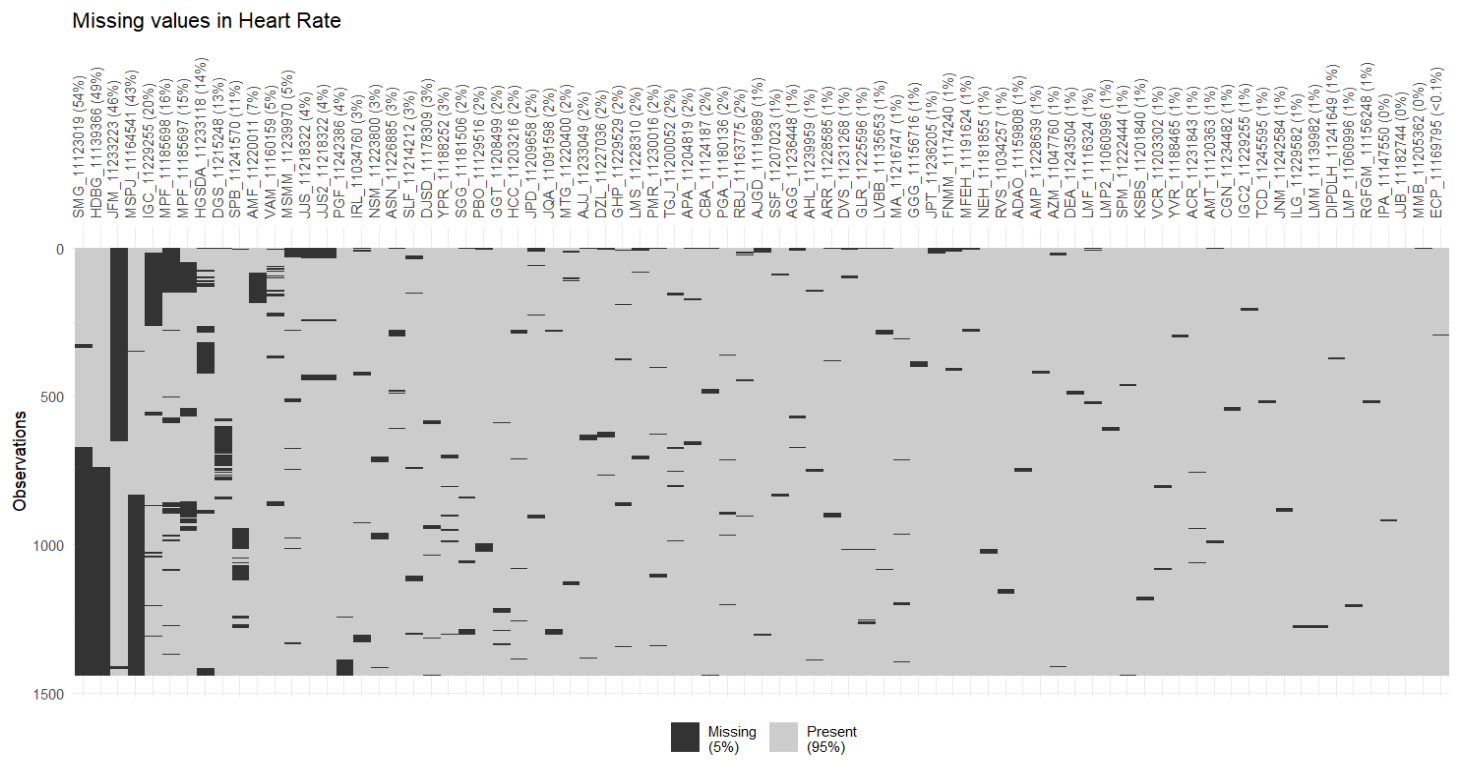
\includegraphics[scale = 0.9]{./img/missing-data-HR.png}
        \caption{Datos Faltantes en la \textit{Frecuencia Cardiaca} de los 79 pacientes pediátricos}
        \label{fig:missing-FC}
    \end{figure}
    
% Se devuelve el formato y la geometría de la página a sus valores originales:
\end{landscape}
\restoregeometry 

\newpage
\thispagestyle{empty}

% Se modifica la geometría (los márgenes) de la página y se coloca en formato horizontal:
\newgeometry{top=10mm, bottom=10mm, left=12mm, right=12mm}
\begin{landscape}

    \begin{figure}[H]
        \centering
        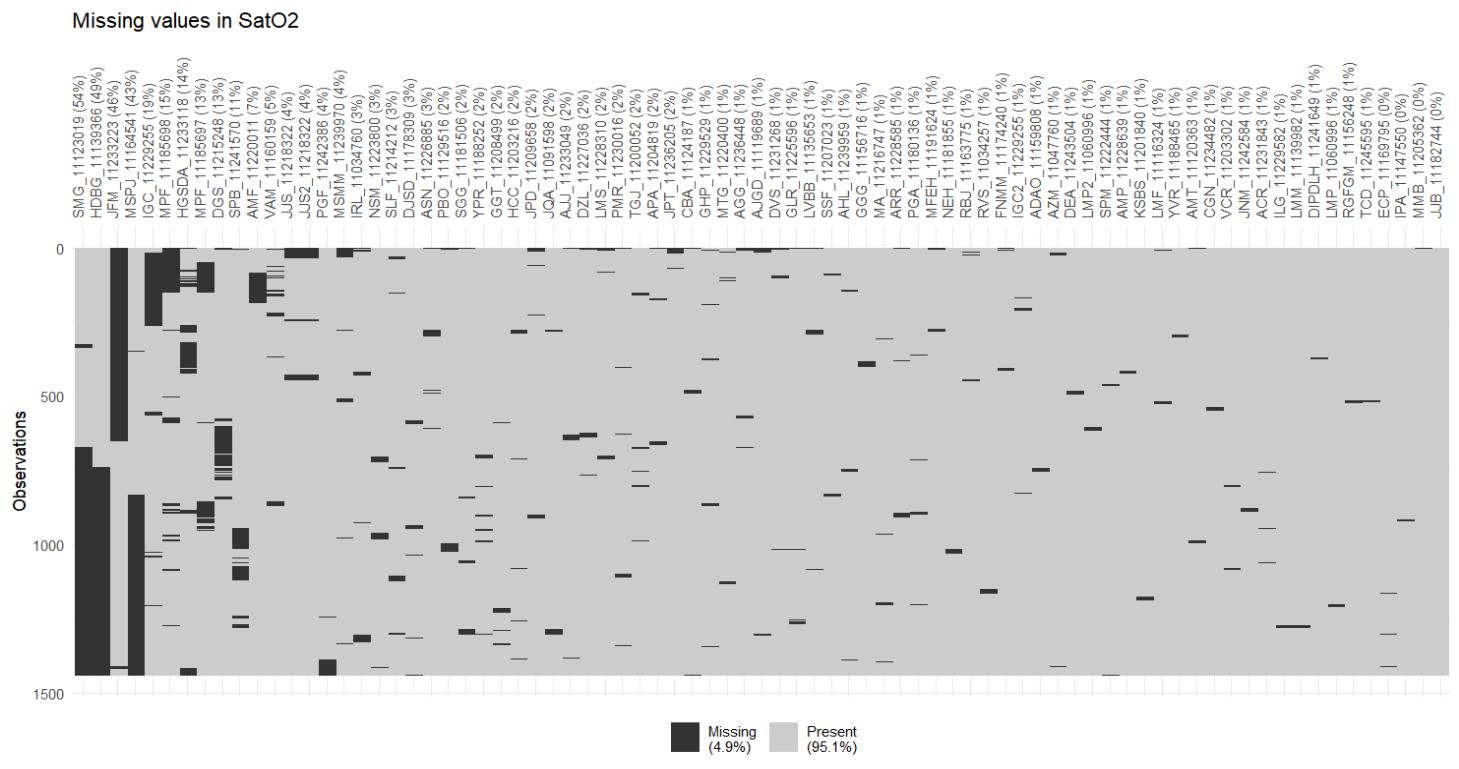
\includegraphics[scale = 0.9]{./img/missing-data-SatO2.png}
        \caption{Datos Faltantes en la \textit{Saturación de O$_2$} de los 79 pacientes pediátricos}
        \label{fig:missing-SatO2}
    \end{figure}
    
% Se devuelve el formato y la geometría de la página a sus valores originales:
\end{landscape}
\restoregeometry 

\paragraph{Selección de Pacientes Válidos}\label{sec:seleccion_pacientes}

 A la hora de determinar los pacientes que van a ser incluidos en el presente \textit{Trabajo de Fin de Máster} se va a tener en cuenta la variable generada y contrastada con los médicos pediatras: \textit{Deterioro}. Esta variable indica si el paciente ha sufrido un deterioro durante las primeras $24$ h de ingreso considerándose \textit{deterioro} si el paciente ha sido trasladado a la UCIP o ha recibido Oxigenación de Alto Flujo. 

 Estudiando los datos se ve como todos los pacientes que han sido trasladados a la UCIP han tenido previamente una intervención en la que se les ha aplicado Oxigenación de Alto Flujo pero no a todos a los que se les ha aplicado Oxigenación de Alto Flujo han sido trasladados a la UCIP. De esta forma los pacientes que muestren \textit{Deterioro} serán los mismos a los que se les ha aplicado OAF. Esto se puede ver en el diagrama de Venn en la Figura \ref{fig:venn-OAF-UCIP}.

\begin{figure}[H]
    \centering
    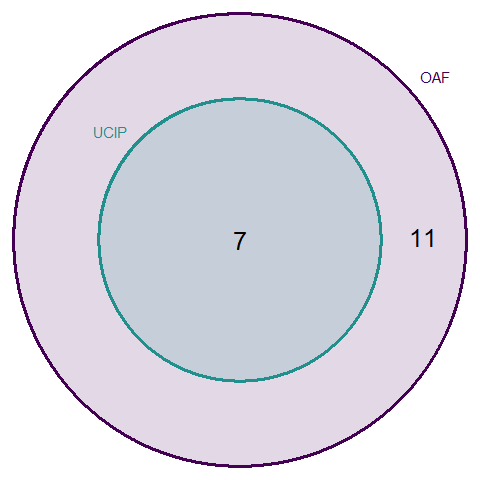
\includegraphics[scale = 1.50]{./img/venn-diagram-OAF-UCIP.png}
    \caption{Diagrama de Venn de los pacientes que han sido trasladados a la UCIP 7 y los que han recibido OAF $11 + 7 = 18$}
    \label{fig:venn-OAF-UCIP}
\end{figure}


A la hora de eliminar pacientes del estudio por su alto porcentaje de valores faltantes, será interesante ver cómo afecta también a la proporción de pacientes que han sufrido \textit{Deterioro} y los que no. En la siguiente Tabla \ref{tabla:ratio-deterioro} se muestra la cantidad de pacientes que presentan \textit{Deterioro}, los que no y el ratio entre \textit{Deterioro} y no \textit{Deterioro} del conjunto total de $79$ pacientes.

\begin{table}[H]
    \centering
    \begin{tabular}{|m{2cm}|m{2.25cm}|m{2cm}|m{2cm}|}
    \hline
        Pacientes Totales & No Deterioro & Deterioro & Ratio \\ \hline
        79 & 61 & 18 & 0.295082 \\ \hline
    \end{tabular}
    \caption{Pacientes Totales, con Deterioro, sin Deterioro y Ratio entre Deterioro y No Deterioro}
        \label{tabla:ratio-deterioro}
\end{table}

\newpage

\subparagraph{Metodologías Exclusión de Pacientes}\label{sec:metodologias_exclusion_pacientes}

Se van a plantear $2$ metodologías para establecer la exclusión de pacientes en el estudio en función de las variables \textit{Series Temporales} de \textit{Frecuencia Cardiaca} y \textit{Saturación de O$_2$}. El objetivo es ver cómo varían la cantidad de pacientes incluidos en el estudio en ambos casos. Un paciente será incluido en el estudio si en las primeras horas establecidas su porcentaje de valores faltantes está por debajo de un \textit{threshold} definido previamente. A continuación se muestran los dos métodos propuestos: 

\begin{itemize}
    \item \textbf{Método 1:} Se va a ir aumentando progresivamente el \textit{threshold} de valores faltantes desde el $5 \%$ hasta el $20 \%$ en intervalos de $2.5 \%$.  Es decir se va a estudiar si existen más pacientes que cumplen el criterio de admisión en las primeras $24$ horas cambiando el \textit{threshold}. Este método se puede ver en la Figura \ref{fig:metodo1}.
    \item \textbf{Método 2:} Se va a establecer un \textit{threshold} en el $5 \%$ de valores faltantes. Una vez establecido dicho \textit{threshold} se va a ir aumentando el tiempo de \textit{scope} del estudio. Es decir, en vez de plantear estudiar las $24$ primeras horas como se ha planteado en el \textit{Método 1}, se va a estudiar si centrándose en un intervalo menor de estudio existen más pacientes que cumplen este criterio de admisión. Se va a ir aumentando el intervalo de estudio desde las $8$ primeras h en intervalos de $30$ minutos hasta las primeras $15$ horas. Es decir se va a estudiar si existen más pacientes que cumplen el criterio de admisión en las primeras $8$ horas, en las primeras $8.5$ horas, en las primeras $9$ horas, etc. hasta llegar a las $15$ primeras horas. Este método se puede ver en la Figura \ref{fig:metodo2}.
\end{itemize}

\begin{figure}[H]
    \centering
    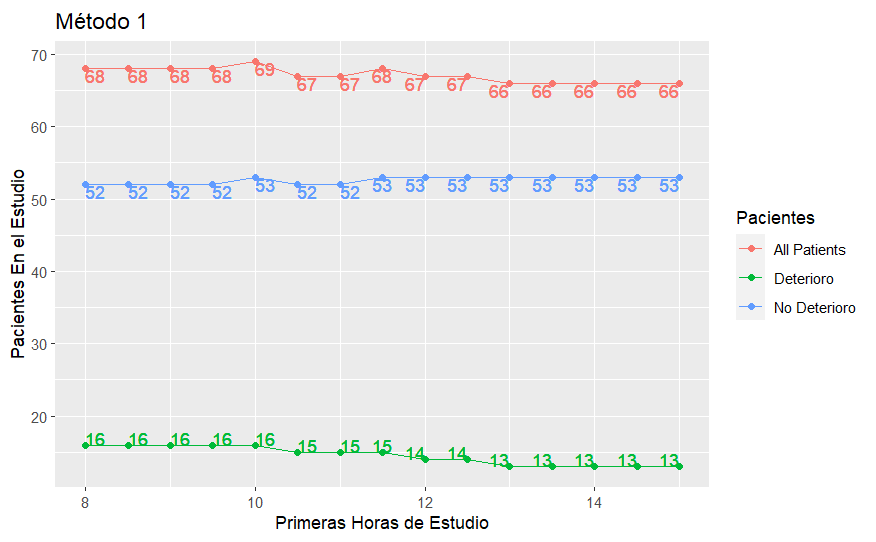
\includegraphics[scale = 1]{./img/metodo1.png}
    \caption{Método 1 de Exclusión de Pacientes}
    \label{fig:metodo1}
\end{figure}

\begin{figure}[H]
    \centering
    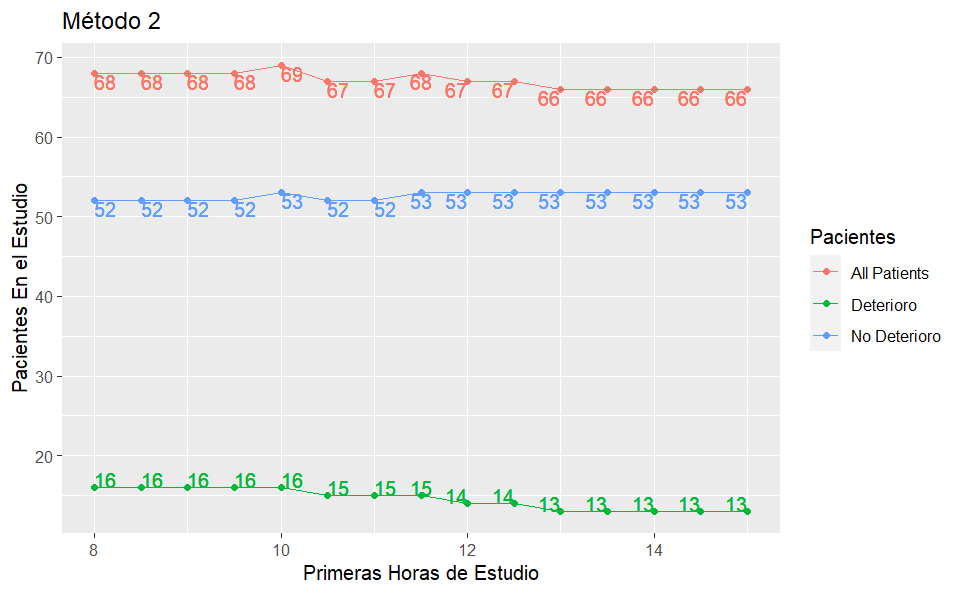
\includegraphics[scale = 1]{./img/metodo2.png}
    \caption{Método 2 de Exclusión de Pacientes}
    \label{fig:metodo2}
\end{figure}

Con los anteriores métodos se ha podido observar cómo realmente el hecho de ser más restrictivos con los datos faltantes no implica que se vayan a excluir muchos más pacientes, y el cambio del ratio $\frac{\textit{Pacientes con Deterioro}}{\textit{Pacientes No Deterioro}}$ es casi inapreciable. Por lo tanto, los datos faltantes se acumulan en un número concreto de pacientes a los que el seguimiento se les ha interrumpido en mayor medida.

En la situación más restrictiva del \textit{Método 1} de la Figura \ref{fig:metodo1} el ratio es de $ \frac{14}{54} \approx 0.26$ y en la menos restrictiva es de $ \frac{16}{59} \approx 0.272$. Cabe decir que la situación más restrictiva es aquella que en las primeras $24$ horas se pide que haya un menor porcentaje de valores faltantes, es decir la combinación de valores más a la izquierda en el eje $x$ de la Figura \ref{fig:metodo1}. Este método muestra un aumento de la muestra de casi un $10 \%$ si se opta por la opción menos restrictiva respecto a la más restrictiva, se pasa de $68$ pacientes a $75$ pacientes totales. 

Por otro lado en la situación más restrictiva del \textit{Método 2} de la Figura~\ref{fig:metodo2} el ratio es de $ \frac{16}{52} \approx 0.307$ y en la situación menos restrictiva el ratio es de $ \frac{13}{53} \approx 0.245$. La variación total de pacientes a incluir en el estudio es de apenas un $3 \%$, se pasa de $68$ pacientes a excluir a $2$ en la situación más restrictiva, obteniendo un total de $66$ pacientes. Cabe aclarar que la situación más restrictiva según este método es aquella que considera más horas de monitorización manteniendo el \textit{threshold} en el $5 \%$ de valores faltantes, es decir la combinación de valores más alejada en el eje $x$ de la Figura \ref{fig:metodo2}.

Para no alterar los datos debido a una posterior imputación y debido a que la variación de los datos es algo considerado como importante en el estudio, se optará por establecer el \textit{threshold} en el $5 \%$ de valores faltantes, haciendo referencia a la siguiente entrada bibliográfica: \cite{Scheffer2002}. 

Junto con este último criterio mencionado se van a hacer dos grupos de pacientes a la hora de hacer el estudio planteado por el presente Trabajo de Fin de Máster, cada grupo de pacientes generado seguirá unas ciertas indicaciones lo que permitirá plantear dos estudios con diferentes objetivos:

\begin{itemize}
    \item \textbf{Valid\_patients\_P1:} Serán aquellos que en las primeras $24$ horas de monitorización tengan un porcentaje de valores faltantes por debajo del $5\%$. Estos pacientes serán aquellos que sigan el criterio más restrictivo del \textit{Método 1} de la Figura \ref{fig:metodo1}. 
    \begin{table}[H]
        \centering
        \begin{tabular}{|m{2cm}|m{2.25cm}|m{2cm}|m{2cm}|}
        \hline
            Pacientes Totales & No Deterioro & Deterioro & Ratio \\ \hline
            68 & 54 & 14 & 0.26 \\ \hline
        \end{tabular}
        \caption{Pacientes Totales, con Deterioro, sin Deterioro y Ratio entre Deterioro y No Deterioro seleccionados para el estudio según el \textit{Método 1}}\label{tabla:ratio-deterioro-P1}
    \end{table}
    \item \textbf{Valid\_patients\_P2:} Serán aquellos que en las primeras $8$ horas de monitorización tengan un porcentaje de valores faltantes por debajo del $5\%$. Estos pacientes serán aquellos que siguen el criterio más restrictivo del \textit{Método 2} de la Figura \ref{fig:metodo2}. Además, se excluirán aquellos pacientes que hayan presentado \textit{Deterioro} en las primeras $8$ horas de monitorización. Esto será así, pues se pretende predecir en las primeras $8$ horas qué pacientes son los que van a presentar \textit{Deterioro} en las siguientes.
    \begin{table}[H]
        \centering
        \begin{tabular}{|m{2cm}|m{2.25cm}|m{2cm}|m{2cm}|}
        \hline
            Pacientes Totales & No Deterioro & Deterioro & Ratio \\ \hline
            58 & 52 & 6 & 0.115 \\ \hline
        \end{tabular}
        \caption{Pacientes Totales, con Deterioro, sin Deterioro y Ratio entre Deterioro y No Deterioro seleccionados para el estudio según el \textit{Método 2} y exclusión de pacientes con \textit{Deterioro} en las primeras 8 horas de monitorización}
            \label{tabla:ratio-deterioro-P1}
    \end{table}
\end{itemize}

Se ha decidido pues que se van a realizar $2$ estudios:

\begin{itemize}
    \item \textbf{Estudio 1:} Se estudiarán a los pacientes pediátricos tomando como referencia las primeras $24$ horas de monitorización, se querrá así pues mantener la unidad \textit{día} en el estudio. Se ha visto que reduciendo el \textit{scope} según el \textit{Método 2} no se consigue un aumento de la muestra de pacientes significativa, y por otro lado reducir la restricción de pacientes con valores faltantes por encima del $5\%$ para aumentar la cantidad de pacientes en el estudio, no es recomendable según la referencia \cite{Scheffer2002}.
    \item \textbf{Estudio 2:} Se estudiarán a los pacientes pediátricos tomando como referencia las primeras $8$ horas de monitorización y excluyendo a aquellos pacientes que han presentado OAF en esas 8 primeras horas así como las variables que se registran más tarde de las $8$ primeras horas. Se ha decidido utilizar las primeras $8$ horas de monitorización ya que se pretende predecir en las primeras $8$ horas qué pacientes son los que van a presentar \textit{Deterioro} en las siguientes próximas horas.
\end{itemize}

\newpage
\subsubsection{Imputación de Datos}\label{sec:imputacion-de-datos}

Una vez que se han decidido los pacientes que se van a incluir tanto en el \textit{Estudio 1} como en el \textit{Estudio 2} se ha de realizar una imputación de datos para permitir a los algoritmos de clasificación discreta poder trabajar con el total de los pacientes, no solo con aquellos que no muestran datos faltantes. 

La imputación de datos se hará en dos documentos diferentes:
\begin{itemize}
    \item \textbf{Archivo de Datos de Pacientes:} En este archivo se imputarán los datos faltantes de las variables \textit{Cuantitativas} y \textit{Cualitativas} de la Tabla~\ref{tabla:cuali_cuanti} mediante el método de la \textit{distancia de Gower}.
    \item \textbf{Carpeta de Datos de Monitorización:} En esta carpeta se imputarán los datos numéricos faltantes de las variables \textit{Series Temporales} que aparecen referenciadas en la Tabla~\ref{tabla:variables_estudio} mediante el método de \textit{k-Nearest Neighbor Imputation}.
\end{itemize}

Cada imputación se hará de una manera diferente. En el primer caso ya que es necesario imputar datos de variables cualitativas y cuantitativas se utilizará el método de \textit{Distancia de Gower}, Sección~\ref{sec:gower_distance} y en el segundo caso se utilizará el método de \textit{k-Nearest Neighbor Imputation}, Sección~\ref{sec:k_Nearest Neighbor_Imputation} ya que muestra mejores resultado a la hora de solo imputar solo variables numéricas.

En el caso de la Frecuencia Cardiaca se realizará una transformación a la cual más tarde se le imputarán datos y se utilizarán como parte del \textit{Estudio 2}. Se hablará de esta transformación más adelante en la Sección~\ref{sec:transformaciones-de-datos}. La imputación de datos se hará una vez realizada la transformación, es decir de \textit{Frecuencia Cardiaca} de cada paciente válido para el estudio en cuestión.

\paragraph{Distancia de Gower}\label{sec:gower_distance}

La \textit{distancia de Gower} puede utilizarse para medir la diferencia entre dos registros que pueden contener una combinación de datos lógicos, numéricos, categóricos o textuales. La distancia es siempre un número comprendido entre 0 (idéntico) y 1 (máxima diferencia). La \textit{distancia de Gower} se calcula como el promedio de las disimilitudes parciales entre individuos. Cuanto menor es el número, más similares son los individuos.

El coeficiente de disimilitud como lo define Gower en su artículo puede ser utilizado para medir la distancia entre dos puntos en un espacio multidimensional y puede ser calculado utilizando diferentes métodos; dependiendo del tipo de datos y del espacio en el que se encuentran los puntos. (~\cite{Gower1971}~)

La imputación de datos se realiza según el código programado que se muestra en la Sección:~\ref{sec:codigo-input-gower}. El código funciona de la siguiente forma: 
\begin{enumerate}
    \item Antes de nada es necesario seleccionar e introducir en la función los siguientes parámetros formales: 
    \begin{itemize}
        \item \texttt{dat}: El conjunto de datos que van a ser utilizados para la imputación (no deben tener datos faltantes). Es decir existe un subconjunto de datos del conjunto de datos total que se utiliza como base de imputación y es de dónde se calculan las distancias respecto al nuevo paciente al que se le quieren imputar datos.
        \item \texttt{new\_with\_null}: El paciente al que se le quieren imputar datos. Dicho paciente se introduce en la función con sus valores faltantes.
        \item \texttt{n\_primeros}: La cantidad $k$ de \textit{vecinos} que se van a tener en cuenta en relación con el paciente al que se le quieren imputar datos. En el caso de este estudio se ha establecido en 5 vecinos, es necesario que sea impar para que la mediana en los datos cualitativos de dos factores con dos opciones se decante por una, cuando hay más factores la situación se complica. 
    \end{itemize}
    \item En segundo lugar se calcula la distancia de Gower entre el paciente seleccionado y el resto de pacientes teniendo solo en cuenta las variables sin datos faltantes. La distancia se calcula entre los pacientes que tienen datos en las variables que se quieren imputar.
    \item Se separan las variables con datos faltantes en cualitativas y cuantitativas, y se seleccionan los $k$ pacientes más parecidos.
    \item Se calcula la media de los valores de las variables cuantitativas de los $k$ pacientes más parecidos y se imputan en el paciente seleccionado.
    \item Se calcula la mediana de los valores de las variables cualitativas de los $k$ pacientes más parecidos y se imputan en el paciente seleccionado.
\end{enumerate}

Es necesario cuando se tiene un conjunto de datos con mezcla de pacientes con valores faltantes hacer un preprocesamiento de los datos para la correcta imputación. Ese preprocesamiento consta de dos pasos: 
\begin{itemize}
    \item \textbf{Separar los pacientes con datos completos de los que no:} Se separan los pacientes con datos completos de los que no. Los pacientes con datos completos se utilizan para imputar a los pacientes don datos faltantes.
    \item \textbf{Imputar sucesivamente:} Se imputan sucesivamente los pacientes con datos faltantes. Es decir, se imputan los datos de un paciente con datos faltantes y se añade a la lista de pacientes con datos completos, separada de la utilizada para imputación. Se ha decidido que nunca se utilizará un paciente con datos imputados para imputar a otro paciente.
\end{itemize}

Los códigos programados que siguen la lógica anteriormente descrita y utilizados para la imputación por este método de la distancia de Gower se encuentran en la Sección~\ref{sec:codigo-input-gower-fun-preprocesamiento}.

El diagrama de flujo dónde se explica lo anteriormente descrito es el siguiente: 

\newpage
\thispagestyle{empty}

% Se modifica la geometría (los márgenes) de la página y se coloca en formato horizontal:
\newgeometry{top=10mm, bottom=10mm, left=12mm, right=12mm}
\begin{landscape}
    \begin{figure}[H]
        \centering
        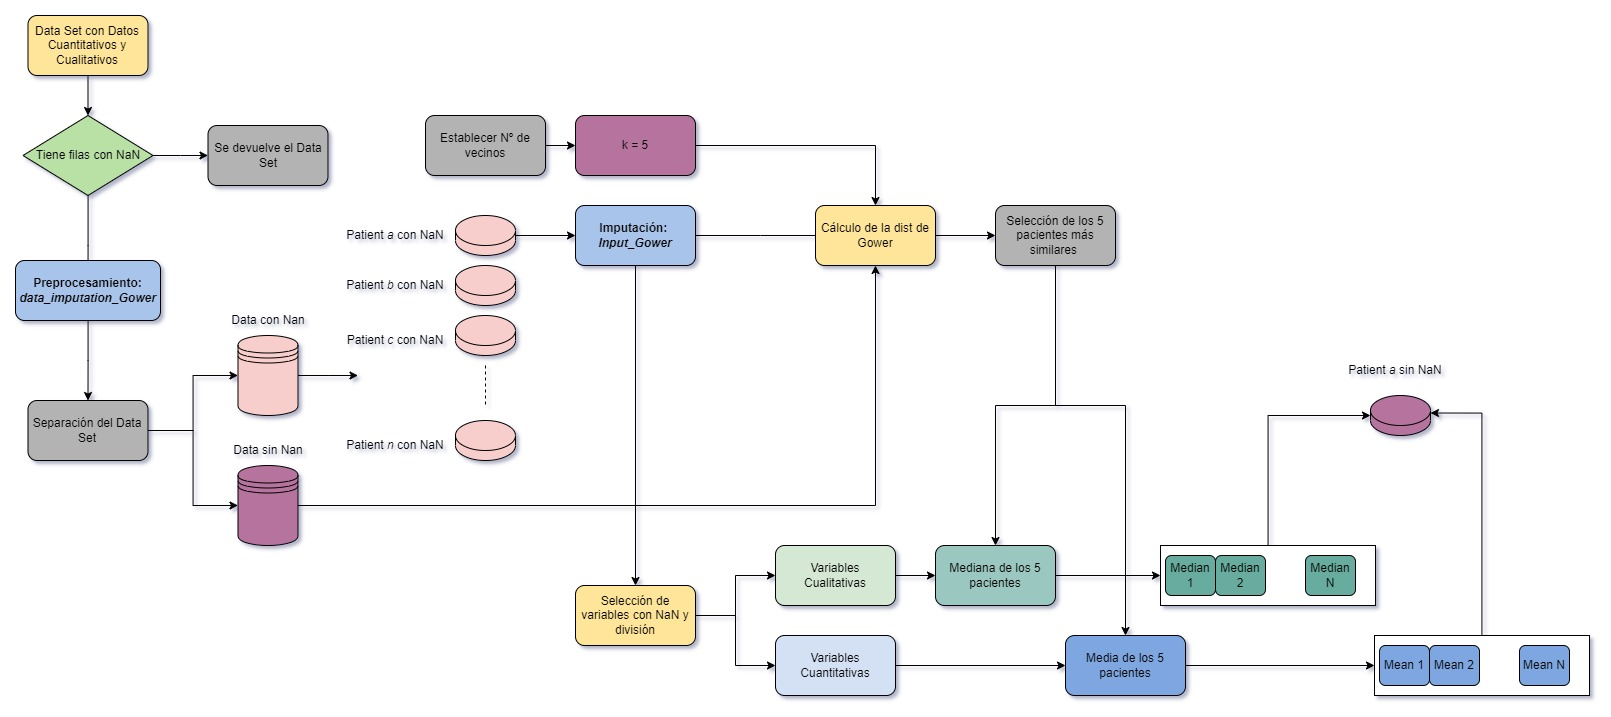
\includegraphics[scale = 0.5]{./img/gower-diagram.jpg}
        \caption{Diagrama de Flujo Imputación por el método de la distancia de Gower}
        \label{fig:gower-diagram}
    \end{figure}
% Se devuelve el formato y la geometría de la página a sus valores originales:
\end{landscape}
\restoregeometry 



\paragraph{k-Nearest Neighbor Imputation}\label{sec:k_Nearest Neighbor_Imputation}

El método de \textit{k-Nearest Neighbor Imputation} al igual que la distancia de Gower es un método de imputación de datos que se basa en la distancia entre los pacientes. Este método se fundamenta en la premisa de que los pacientes que son similares presentan valores parecidos en las variables que se desean imputar. En este caso se ha utilizado el paquete \texttt{DMwR2} de \texttt{R} para realizar la imputación.~(\cite{DMwR2}).

La imputación \textit{k-Nearest Neighbor Imputation} es un método utilizado para rellenar los valores que faltan en un conjunto de datos utilizando los valores de los $k$ vecinos más próximos. Este método es especialmente útil para variables numéricas, en las que los valores que faltan pueden sustituirse por la media de los $k$ vecinos más próximos.

La ventaja de este método respecto a la \textit{distancia de Gower} es que aparte de que ya viene construido el algoritmo de imputación en el paquete de Rstudio \textit{DMwR2}, es que solo se imputarán datos numéricos y para esta casuística es método más adecuado y programado orientado a este objetivo.

Un ejemplo que ilustra este enfoque de imputación se encuentra en el estudio titulado \textit{Missing Data Imputation for Geolocation-based Price Prediction Using KNN MCF Method} \cite{Sanjar2020}. En este trabajo, se empleó la técnica de imputación conocida como \textit{k-Nearest Neighbor Imputation}, lo cual permitió mejorar significativamente la precisión del modelo y evitar problemas de sobreajuste. El método propuesto alcanzó una precisión de predicción del $92.01$\%, con la asistencia del algoritmo de clasificación \textit{Random Forest}.

La función usada de imputación usará los $5$ vecinos más cercanos y el método de imputación es el de la media ponderada de los vecinos más cercanos \textit{weighAvg}. La función de imputación una vez que identifica los k vecinos más cercanos, calculan los pesos para cada uno de ellos en función de la distancia a la observación original que tiene el valor al faltante. Los vecinos más cercanos tienen mayor influencia a la hora de la imputación debido a sus mayores pesos. La media ponderada se utiliza como el valor imputado para el dato faltante en la observación original. La función usada para la imputación es la siguiente referenciada en el Código~\ref{cod:snipet-knn-impute}:

\begin{code}[H]
\begin{lstlisting}
    knnImputation(data, k = 5, scale = T, meth = "weighAvg",
    distData = NULL)
\end{lstlisting}
\caption{Código KNN Impute Función}
\label{cod:snipet-knn-impute}
\end{code}

Respecto a los valores imputados mediante este método serán los valores faltantes de las \textit{Series Temporales} referenciados en la Tabla~\ref{tabla:variables_estudio} y sus respectivas transformaciones sobre las que más tarde se hablará de ellas en la Sección~\ref{sec:transformaciones-de-datos}. 

A la hora de imputar datos cabe diferenciar entre los dos Estudios realizados. Cada estudio considera unos pacientes en un intervalo de tiempo diferente. Debido a esta casuística se ha decidido imputar los datos de los pacientes de cada estudio por separado. Es decir, se imputarán los datos de los pacientes del \textit{Estudio 1} por un lado y los del \textit{Estudio 2} por otro.

\subparagraph*{Diagrama de imputación de datos de \textit{Series Temporales} por el método de imputación \textit{k-Nearest Neighbor Imputation}}\label{sec:diagrama-imputacion-knn} \\

Cada paciente será estudiado de manera individualizada. Esto implica que los datos de monitorización de cada \textit{Series Temporal} en referencia a cada paciente se tienen que dividir en diferentes en franjas horarias para así realizar la imputación de datos. Estas franjas horarias dependerá del tipo de estudio. En el \textit{Estudio 1} las franjas horarias serán $40$ de $36$ minutos cada una lo que hace un total de $1440$ minutos que son justamente las $24$ horas de estudio, Figura~\ref{fig:knn-diagram-e1}. En el \textit{Estudio 2} las franjas horarias serán $20$ de $24$ minutos lo que hace un total de $480$ minutos que son justamente las $8$ horas de estudio, Figura~\ref{fig:knn-diagram-e2}.

Una vez que se han dividido los datos de cada paciente en franjas horarias se imputarán los datos de cada franja horaria por separado. Es decir, se imputarán los datos de la primera franja horaria de cada paciente en relación con las 5 más cercanas, después los de la segunda, etc, así hasta llegar a la última franja horaria de cada paciente. Es obvio que solo se imputarán datos de las franjas horarias que tengan datos faltantes y se utilizarán las $5$ franjas horarias más cercanas que tengan datos en el minuto que se quiera imputar.

\newpage
\thispagestyle{empty}
% Se modifica la geometría (los márgenes) de la página y se coloca en formato horizontal:
\newgeometry{top=10mm, bottom=10mm, left=12mm, right=12mm}
\begin{landscape}
    \begin{figure}[H]
        \centering
        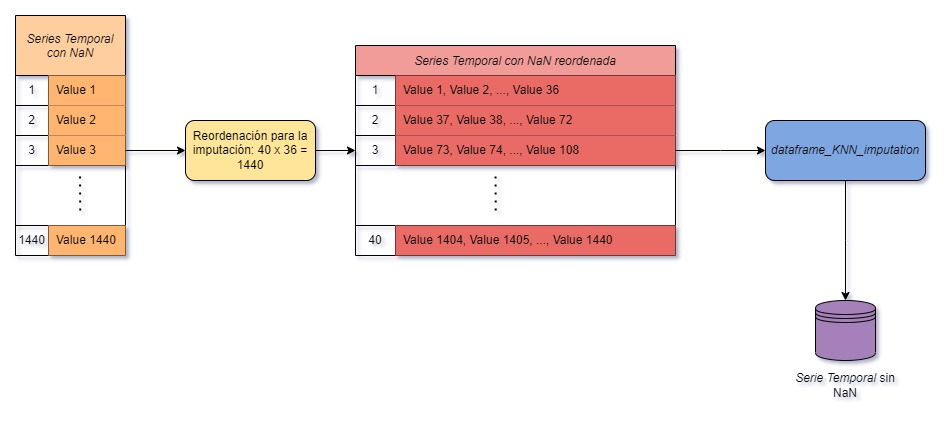
\includegraphics[scale = 0.5]{./img/knn-diagram-e1.jpg}
        \caption{Diagrama de Flujo Imputación por el método de \textit{k-Nearest Neighbor Imputation} según el \textit{Estudio 1}}
        \label{fig:knn-diagram-e1}
    \end{figure}
    \begin{figure}[H]
        \centering
        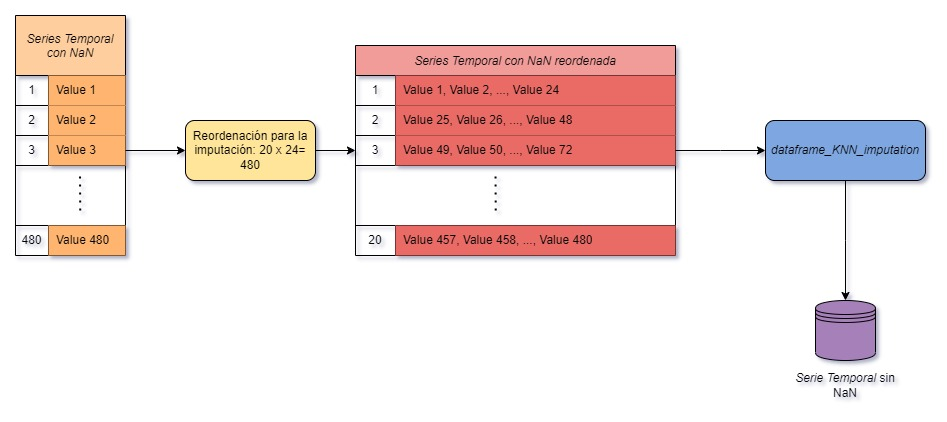
\includegraphics[scale = 0.5]{./img/knn-diagram-e2.jpg}
        \caption{Diagrama de Flujo Imputación por el método de \textit{k-Nearest Neighbor Imputation} según el \textit{Estudio 2}}
        \label{fig:knn-diagram-e2}
    \end{figure}
% Se devuelve el formato y la geometría de la página a sus valores originales:
\end{landscape}
\restoregeometry 

\newpage
\subsubsection{Transformaciones de los Datos}\label{sec:transformaciones-de-datos}

En el presente \textit{Trabajo de Fin de Máster} se ha pretendido eliminar el componente \textit{EDAD} de los datos de monitorización de los pacientes pediátricos. Esto se ha hecho por dos motivos, el primero es que a la hora de realizar clusters no queremos dividir los pacientes por \textit{PESO} y \textit{EDAD}, se quieren buscar otras variable que permitan hacer grupos, el segundo es que los algoritmos de clasificación discreta utilizados (\textit{Random Forest}) no se centren en la edad del paciente a la hora de predecir si el paciente va a presentar \textit{Deterioro} o no, será una variable de entrada pero se quiere reducir el peso decisivo en ella.

Se van a plantear dos formas de eliminar este efecto.

\paragraph{Eliminar la Componente \textit{EDAD} de los Datos de Monitorización de los Pacientes Pediátricos Mediante la Transformación Cuantílica de los Datos}\label{sec:eliminar-edad-1} \\

Para eliminar este componente, se ha recurrido al estudio~\cite{percentilesFenton2015}, el cual recoge los valores de \textit{Frecuencia Cardiaca} y \textit{Frecuencia Respiratoria}  de varios pacientes pediátricos y los organiza por percentiles, este estudio recoge datos de pacientes que acudieron a un servicio de urgencias pediátrico en un hospital australiano. Se utilizarán de dicho estudio los valores en referencia a la \textit{Frecuencia Cardiaca}. A continuación se muestran los valores de \textit{Frecuencia Cardiaca} en función de la \textit{Edad} en la Tabla~\ref{tabla:age_percentiles}:

\newpage
\thispagestyle{empty}
% Se modifica la geometría (los márgenes) de la página y se coloca en formato horizontal:
\newgeometry{top=10mm, bottom=10mm, left=12mm, right=12mm}
\begin{landscape}
    \begin{table}[htbp]
        \centering
        \caption{Percentiles de \textit{Frecuencia Cardiaca} en función de la \textit{Edad} (~\cite{percentilesFenton2015})}
        \label{tabla:age_percentiles}
        \begin{tabular}{|l|l|l|l|l|l|l|l|l|l|l|l|}
            \toprule
            Age & Age\_0 & {Amount} & {1st} & {5th} & {10th} & {25th} & {50th} & {75th} & {90th} & {95th} & {99th} \\
            \midrule
            0--$<$3 months & months & 3365,00 & 109,00 & 119,00 & 123,00 & 132,00 & 142,00 & 154,00 & 165,00 & 171,00 & 181,00 \\
            3--$<$6 months & months & 4493,00 & 100,00 & 113,00 & 118,00 & 124,00 & 135,00 & 145,00 & 155,00 & 161,00 & 174,00 \\
            6--$<$9 months & months & 5927,00 & 100,00 & 110,00 & 115,00 & 121,00 & 131,00 & 141,00 & 151,00 & 159,00 & 172,00 \\
            10--$<$12 months & months & 6005,00 & 98,00 & 105,00 & 111,00 & 119,00 & 127,00 & 139,00 & 150,00 & 160,00 & 174,00 \\
            12--$<$18 months & months & 10,00 & 94,00 & 101,00 & 107,00 & 116,00 & 124,00 & 136,00 & 149,00 & 159,00 & 176,00 \\
            18--$<$24 months & months & 9370,00 & 90,00 & 99,00 & 103,00 & 112,00 & 120,00 & 132,00 & 145,00 & 154,00 & 172,00 \\
            2--$<$3 years & years & 15,00 & 85,00 & 96,00 & 99,00 & 107,00 & 117,00 & 126,00 & 138,00 & 146,00 & 162,00 \\
            3--$<$4 years & years & 11,00 & 80,00 & 89,00 & 94,00 & 102,00 & 111,00 & 121,00 & 131,00 & 138,00 & 152,00 \\
            4--$<$6 years & years & 15,00 & 74,00 & 82,00 & 88,00 & 96,00 & 105,00 & 117,00 & 126,00 & 133,00 & 146,00 \\
            6--$<$8 years & years & 9100,00 & 69,00 & 78,00 & 81,00 & 90,00 & 100,00 & 111,00 & 122,00 & 128,00 & 141,00 \\
            8--$<$12 years & years & 12,00 & 64,00 & 72,00 & 77,00 & 84,00 & 94,00 & 104,00 & 116,00 & 122,00 & 135,00 \\
            12--$<$15 years & years & 6054,00 & 59,00 & 64,00 & 69,00 & 77,00 & 86,00 & 97,00 & 106,00 & 113,00 & 127,00 \\
            15--$<$16 years & years & 1339,00 & 56,00 & 62,00 & 66,00 & 74,00 & 83,00 & 94,00 & 103,00 & 111,00 & 122,00 \\
            \bottomrule
        \end{tabular}
    \end{table}
\end{landscape}
\restoregeometry 

Para esta transformación lo primero que se ha realizado es; partir de la Tabla~\ref{tabla:age_percentiles}. Gracias a esta tabla, se han generado distribuciones normales para cada uno de los percentiles de la \textit{Frecuencia Cardiaca} en función de la \textit{Edad}. Para ello se ha utilizado la función \texttt{get.norm.par} del paquete de R \texttt{rriskDistributions} que genera distribuciones normales a partir de los percentiles y los valores cuantílicos, es decir el valor que se tiene en ese percentil (~\cite{rriskDistributions}). Se utilizará el siguiente \textit{snippet} de Código~\ref{cod:snipet-generate-norm-distributions} para generar las distribuciones normales de cada uno de los percentiles:

\begin{itemize}
    \item \texttt{cuantiles\_HR}: Es la Tabla \ref{tabla:age_percentiles}.
    \item \texttt{param\_norm\_heart\_rate}: Es la tabla que contiene las distribuciones normales generadas a partir de la Tabla~\ref{tabla:age_percentiles}.
\end{itemize}

\begin{code}[H]
\begin{lstlisting}
p <- c(0.01,0.05,0.10,0.25,0.50,0.75,0.90,0.95,0.99)

for (i in c(1:dim(cuantiles_HR)[1])) {
  q <- as.numeric(cuantiles_HR[i,4:dim(cuantiles_HR)[2]])
  fit_results <- rriskDistributions::get.norm.par(p = p ,q = q)
  param_norm_heart_rate[i,] <- as.vector(fit_results)
}
\end{lstlisting}
\caption{Código Generación de Distribuciones Normales}
\label{cod:snipet-generate-norm-distributions}
\end{code}

A continuación se muestran las distribuciones normales generadas para cada uno de los percentiles de la \textit{Frecuencia Cardiaca} en función de la \textit{Edad} en la Tabla~\ref{tabla:age_norm_distributions}, dichos valores se almacenan en la variable \texttt{param\_norm\_heart\_rate} en el Código~\ref{cod:snipet-generate-norm-distributions}:

\begin{table}[htbp]
    \centering
    \caption{Valores de las distribuciones normales de \textit{Frecuancia Cardiaca} generadas}
    \label{tabla:age_norm_distributions}
    \begin{tabular}{l S[table-format=3.7] S[table-format=2.8]}
        \toprule
        Age & {Mean} & {SD}  \\ 
        \midrule
        0--$<$3 months & 142.8975133 & 16.106937  \\
        3--$<$6 months & 135.1382501 & 14.79739075  \\
        6--$<$9 months & 131.4553211 & 14.30632493  \\
        10--$<$12 months & 128.5778996 & 15.07784388  \\
        12--$<$18 months & 125.5921228 & 15.61675197  \\
        18--$<$24 months & 121.6350336 & 15.40451936  \\
        2--$<$3 years & 117.0837814 & 14.46325736  \\
        3--$<$4 years & 111.5315149 & 14.3094006  \\
        4--$<$6 years & 106.0971108 & 15.21660598  \\
        6--$<$8 years & 100.6070164 & 15.48392466  \\
        8--$<$12 years & 94.46367306 & 14.81625947  \\
        12--$<$15 years & 86.81086606 & 14.53201736  \\
        15--$<$16 years & 83.84981343 & 14.47422122  \\
        \bottomrule
    \end{tabular}
\end{table}

Una vez que se han obtenido las distribuciones normales de cada uno de los rangos de edad se ha realizado la transformación de los datos de cada paciente en función de sus valores de \textit{Frecuencia Cardiaca} en cada momento ed la monitorización. Es decir, a cada paciente se le asignará una distribución normal en función de su edad de las que se muestran en la Tabla~\ref{tabla:age_norm_distributions}.

Para ello se ha utilizado la función \texttt{pnorm} de \texttt{R} que calcula el percentil al que pertenece un valor en función de la distribución normal referente a la edad dada.  A continuación se muestra el código de la transformación de los datos de cada paciente en función de sus valores de \textit{Edad} y \textit{Frecuencia Cardiaca}: 

\begin{itemize}
    \item \texttt{FC\_all\_patients\_t}: Este \texttt{data.frame} contiene los datos traspuestos de \textit{Frecuencia Cardiaca} de todos los pacientes válidos para el estudio en cuestión, cada paciente sería una columna de dicho \texttt{data.frame} y cada fila un valor de monitorización. A este \texttt{data.frame} traspuesto se le añade al final una nueva columna que contiene la \textit{Edad} de cada paciente.
    \item \texttt{cuantiles\_TS\_HR}: Es el nuevo \texttt{data.frame} que se genera con los datos transformados de \textit{Frecuencia Cardiaca}, cada paciente es una columna de dicho \textt{data.frame}. Su dimensión sería $1440$ filas (minutos) y $79$ columnas, una por cada paciente. Es importante destacar que la trasformación se la hace a todos los pacientes, sean válidos o no para los dos estudios planteados. 
\end{itemize}

\begin{code}[H]
    \begin{lstlisting}
    for (name in patient_name) {
        edad = FC_all_patients_t[name , "EDAD"]
        if (edad <= 3) {
            mean_patient = param_norm_heart_rate[1, ]$Mean
            sd_patient = param_norm_heart_rate[1, ]$SD
        } else if (edad <= 6) {
            mean_patient = param_norm_heart_rate[2, ]$Mean
            sd_patient = param_norm_heart_rate[2, ]$SD
        } else if (edad <= 9) {
            mean_patient = param_norm_heart_rate[3, ]$Mean
            sd_patient = param_norm_heart_rate[3, ]$SD
        } else if (edad <= 12) {
            mean_patient = param_norm_heart_rate[4, ]$Mean
            sd_patient = param_norm_heart_rate[4, ]$SD
        } else if (edad <= 18) {
            mean_patient = param_norm_heart_rate[5, ]$Mean
            sd_patient = param_norm_heart_rate[5, ]$SD
        } else if (edad <= 24) {
            mean_patient = param_norm_heart_rate[6, ]$Mean
            sd_patient = param_norm_heart_rate[6, ]$SD
        } else if (edad <= 36) {
            mean_patient = param_norm_heart_rate[7, ]$Mean
            sd_patient = param_norm_heart_rate[7, ]$SD
        } else if (edad <= 48) {
            mean_patient = param_norm_heart_rate[8, ]$Mean
            sd_patient = param_norm_heart_rate[8, ]$SD
        } else if (edad < 72) {
            mean_patient = param_norm_heart_rate[9, ]$Mean
            sd_patient = param_norm_heart_rate[9, ]$SD
        } else {
            mean_patient = param_norm_heart_rate[10, ]$Mean
            sd_patient = param_norm_heart_rate[10, ]$SD
        }
        
        for (i in 1:dim(cuantiles_TS_HR)[1]) {
            cuantiles_TS_HR[i, name] = pnorm(FC_all_patients[i, name], mean = mean_patient, sd = sd_patient)
        }
          }
    }
    \end{lstlisting}
    \caption{Código Transformación de los datos de \textit{Frecuencia Cardiaca} de cada paciente en función de su \textit{Edad}}
    \label{cod:transformación-frecuencia-cardiaca}
\end{code}


Se va a mostrar una visualización de la transformación de todos los datos de \textit{Frecuencia Cardiaca}. Cada valor de cada paciente será etiquetado con la edad de dicho paciente y se mostraran en un gráfico de densidad para cada rango de edad. En la Figura~\ref{fig:transformacion-frecuencia-cardiaca-edad} se muestra el resultado de la transformación realizada según lo descrito en este apartado, de los datos de \textit{Frecuencia Cardiaca} de todos los pacientes en función de su \textit{Edad} y el la Figura~\ref{frecuencia-cardiaca-edad} se muestran los datos de \textit{Frecuencia Cardiaca} de todos los pacientes en función de su \textit{Edad} sin transformar.

\begin{figure}[H]
    \centering
    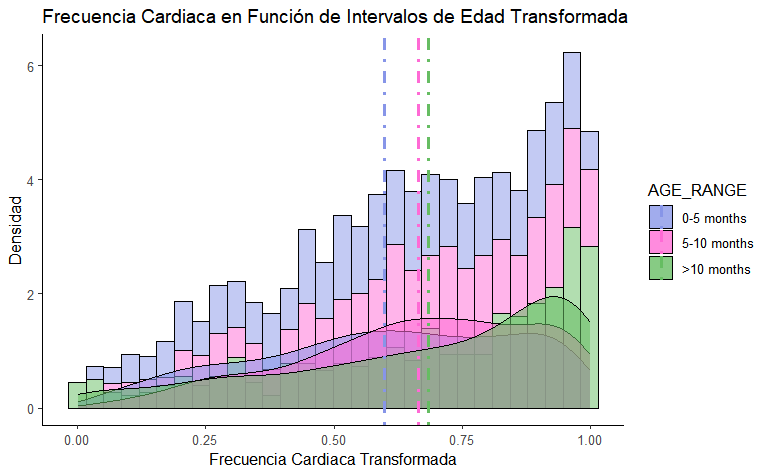
\includegraphics[width=0.9\textwidth]{img/transformacion-frecuencia-cardiaca-edad.png}
    \caption{Transformación de los datos de \textit{Frecuencia Cardiaca} de todos los pacientes en función de su \textit{Edad}}
    \label{fig:transformacion-frecuencia-cardiaca-edad}
\end{figure}

\begin{table}[H]
    \centering
    \begin{tabular}{lcc}
        \toprule
        \textbf{Intervalos de Edad (Meses)} & \textbf{Media} \\
        \midrule
        $0 \leq \text{EDAD} < 5$ & 0.5976350 \\
        $5 \leq \text{EDAD} < 10$ & 0.6632027 \\
        $\text{EDAD} \geq 10$ & 0.6829290 \\
        \bottomrule
    \end{tabular}
    \caption{Valores Promedio de Frecuencia Cardiaca Transformados en Función de la Edad}\label{tabla:frecuencia-cardiaca-edad-transformada}
\end{table}

\begin{figure}[H]
    \centering
    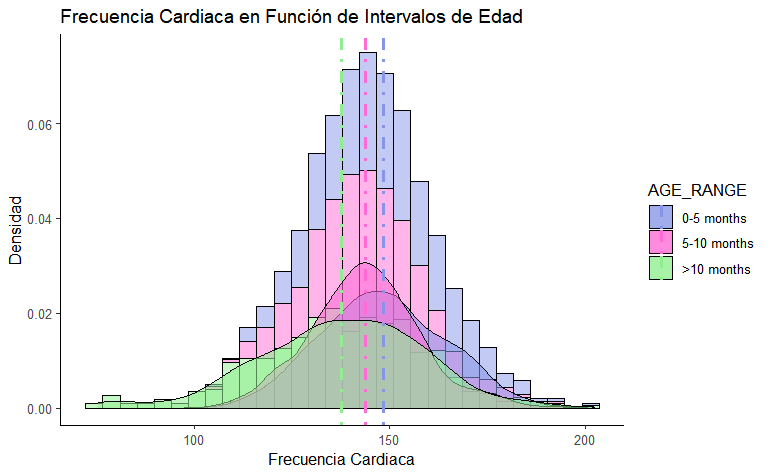
\includegraphics[width=0.9\textwidth]{img/frecuencia-cardiaca-edad.png}
    \caption{Datos de \textit{Frecuencia Cardiaca} de todos los pacientes en función de su \textit{Edad}}
    \label{fig:frecuencia-cardiaca-edad}
\end{figure}

\begin{table}[H]
    \centering
    \begin{tabular}{lcc}
        \toprule
        \textbf{Intervalos de Edad (Meses)} & \textbf{Media} \\
        \midrule
        $0 \leq \text{EDAD} < 5$ & 148.2984 \\
        $5 \leq \text{EDAD} < 10$ & 143.7214 \\
        $\text{EDAD} \geq 10$ & 137.6679 \\
        \bottomrule
    \end{tabular}
    \caption{Valores Promedio de Frecuencia Cardiaca en Función de la Edad}
    \label{tabla:frecuencia-cardiaca-edad}
\end{table}

Al observar que las medias de la Tabla~\ref{tabla:frecuencia-cardiaca-edad-transformada} por \textit{Edad} no concuerdan una vez haber hechas las transformaciones, puede haber dos interpretaciones posibles: o bien los datos recopilados de la fuente~\cite{percentilesFenton2015} no son completamente precisos, o bien existe un intervalo específico de pacientes que experimentan una variabilidad mucho mayor en su \textit{Frecuencia Cardíaca} cuando se enferman dentro de un cuadro con complicaciones respiratorias, lo que afecta significativamente a la media de dicho intervalo.

\paragraph{Eliminar la Componente \textit{EDAD} de los Datos de Monitorización de los Pacientes Pediátricos Mediante la Transformación Escalada de los Datos}\label{sec:eliminar-edad-2} \\

Se va a plantear otra transformación mediante el escalado de los datos para ver si se puede paliar de esta forma el efecto de la \textit{EDAD}. 

Para escalar los datos se deben de realizar dos pasos:

\begin{enumerate}
    \item Calcular la media (\(\bar{x}\)) y la desviación estándar (\(s\)) de los datos de \textit{Frecuencia Cardiaca} de todos los pacientes.
    \[
        \bar{x} = \frac{\sum_{i=1}^{n} x_i}{n}, \quad s = \sqrt{\frac{\sum_{i=1}^{n} (x_i - \bar{x})^2}{n-1}}
    \]

    \item Restar a cada valor de \textit{Frecuencia Cardiaca} de cada paciente la media y dividirlo por la desviación estándar.
    \[
        x_{\text{centered}_{ij}} = x_{ij} - \bar{x}, \quad x_{\text{scaled}_{ij}} = \frac{x_{\text{centered}_{ij}}}{s}
    \]
\end{enumerate}

El proceso de transformación se llevó a cabo utilizando el siguiente código (~\cite{BeckerChambersWilks1988}):

\begin{code}[H]
    \begin{lstlisting}
scale(x, center = TRUE, scale = TRUE)
    \end{lstlisting}
    \caption{Transformación de datos de \textit{Frecuencia Cardiaca} mediante Escalado}\label{cod:transformacion-fc-escalado}
 \end{code}


Una vez realizada esta transformación los resultados son los siguientes: 


\begin{figure}[H]
    \centering
    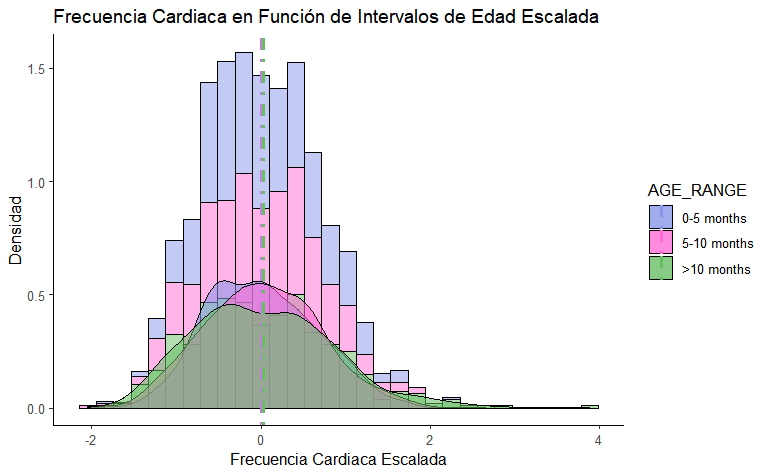
\includegraphics[width=0.9\textwidth]{img/frecuencia-cardiaca-edad-escalada.png}
    \caption{Datos de \textit{Frecuencia Cardiaca} Escalados de todos los pacientes en función de su \textit{Edad}}
    \label{fig:frecuencia-cardiaca-edad-escala}
\end{figure}

\begin{table}[H]
    \centering
    \begin{tabular}{lcc}
        \toprule
        \textbf{Intervalos de Edad (Meses)} & \textbf{Media} \\
        \midrule
        $0 \leq \text{EDAD} < 5$ & 0.01018835 \\
        $5 \leq \text{EDAD} < 10$ & 0.01371264 \\
        $\text{EDAD} \geq 10$ & 0.03299302 \\
        \bottomrule
    \end{tabular}
    \caption{Valores Promedio de Frecuencia Cardiaca Escalados en Función de la Edad}
    \label{tabla:frecuencia-cardiaca-escalada-edad}
\end{table}

En este caso se ha conseguido con mayor éxito eliminar la componente de la \textit{EDAD} de los datos de \textit{Frecuencia Cardiaca} de los pacientes en comparación con la transformación realizada en la Sección~\ref{sec:eliminar-edad-1}.


\newpage
\subsubsection{Análisis Descriptivo}\label{sec:transformaciones-de-datos}

A continuación se muestra el análisis descriptivo de los $79$ pacientes recopilados por el presente \textit{Trabajo de Fin de Máster}. 

\newpage
\thispagestyle{empty}
% Se modifica la geometría (los márgenes) de la página y se coloca en formato horizontal:
\newgeometry{top=10mm, bottom=10mm, left=12mm, right=12mm}
\begin{landscape}
    \begin{table}[h]
        \centering
        \caption{Descripción de Variables}
        \begin{tabular}{lcccccccc}
        \hline
        Variable & EDAD & PESO & EG & PCT & PCR & LEUCOCITOS & NEUTROFILOS & LINFOCITOS \\ \hline
        Min. & 0.30 & 2.81 & 25.0 & 0.0600 & 0.1000 & 6000 & 1800 & 1400 \\
        1st Qu. & 1.80 & 4.38 & 37.0 & 0.1725 & 0.9625 & 8500 & 3300 & 3200 \\
        Median & 4.60 & 6.26 & 39.0 & 0.4250 & 2.5500 & 11600 & 5600 & 4800 \\
        Mean & 6.83 & 6.54 & 37.7 & 1.8725 & 5.4432 & 12188 & 5588 & 4912 \\
        3rd Qu. & 10.85 & 8.65 & 40.0 & 2.8075 & 8.6250 & 14600 & 7400 & 5900 \\
        Max. & 29.00 & 12.00 & 41.0 & 7.5100 & 28.3000 & 22000 & 10900 & 10900 \\ \hline
        Variable & FR\_0\_8h & FR\_8\_16h & FR\_16\_24h & FLUJO2\_0\_8H & FLUJO2\_8\_16h & FLUJO2\_16\_24h \\ \hline
        Min. & 26.00 & 22.00 & 24.00 & 0.000 & 0.000 & 0.000 \\
        1st Qu. & 40.00 & 36.00 & 38.50 & 1.000 & 0.600 & 0.500 \\
        Median & 44.00 & 44.00 & 43.00 & 1.500 & 1.000 & 1.000 \\
        Mean & 46.73 & 44.23 & 44.01 & 1.326 & 1.211 & 1.071 \\
        3rd Qu. & 53.50 & 51.50 & 48.00 & 2.000 & 2.000 & 1.500 \\
        Max. & 96.00 & 68.00 & 68.00 & 3.000 & 3.000 & 3.000 \\ \hline
        \end{tabular}
        \label{tab:datos_descripcion_cuantitativos}
    \end{table}
\end{landscape}
\restoregeometry 
    
\newpage
\thispagestyle{empty}
% Se modifica la geometría (los márgenes) de la página y se coloca en formato horizontal:
\newgeometry{top=10mm, bottom=10mm, left=12mm, right=12mm}
\begin{landscape}
\begin{table}[h]
    \centering
    \caption{Distribución de Variables Categóricas Multicategoría}
    \begin{tabular}{lccc}
    \hline
    ETIOLOGIA & ALIMENTACION & SEXO \\
    \hline
    NO      :33   & ABSOL  : 6    & MASC:42 \\
    VRS     :43   & NORMAL :53    & FEM :37 \\
    COVID   : 0   & SNG/STP:17    & \\
    GRIPE   : 0   & NA's   : 3    & \\
    OTRO    : 3   &                & \\
    VRS+OTRO: 0   &                & \\
    \hline
    \end{tabular}\label{tabla:distribucion_variables_categoricas_multicat}
\end{table}

\begin{table}[h]
    \centering
    \caption{Distribución de Variables Categóricas SI/NO (Part 1)}
    \begin{tabular}{lcccccccc}
    \hline
        ~ & PALIVIZUMAB & LM & DERMATITIS & ALERGIAS & TABACO & ENFERMEDAD\_BASE & RADIOGRAFIA & ANALITICA \\
        \hline
        NO & 73 & 47 & 74 & 71 & 30 & 58 & 58 & 56 \\
        SI & 6 & 32 & 5 & 8 & 36 & 21 & 8 & 23 \\
        NA's & ~ & ~ & ~ & ~ & 13 & ~ & 13 & ~ \\
        \hline
    \end{tabular}
    \label{tabla:distribucion_variables_categoricas_si_no_1}
\end{table}

\begin{table}[h]
    \centering
    \caption{Distribución de Variables Categóricas SI/NO (Part 2)}
    \begin{tabular}{lcccccccc}
    \hline
        ~ & SUERO & SNG & GN\_INGRESO & OAF & OAF\_AL\_INGRESO & OAF\_TRAS\_INGRESO & UCIP & DETERIORO \\
        \hline
        NO & 59 & 64 & 18 & 61 & 74 & 66 & 72 & 61 \\
        SI & 20 & 15 & 57 & 18 & 5 & 13 & 7 & 48 \\
        NA's & ~ & ~ & 4 & ~ & ~ & ~ & ~ & ~ \\
        \hline
    \end{tabular}
    \label{tabla:distribucion_variables_categoricas_si_no_2}
\end{table}

\begin{table}[h]
    \centering
    \caption{Distribución de Variables Categóricas Escalas}
    \begin{tabular}{lcccccc}
    \hline
        ~ & SAPI\_0\_8h & SAPI\_8\_16h & SAPI\_16\_24h & SCORE\_CRUCES\_INGRESO & SCORE\_WOOD\_DOWNES\_INGRESO & SCORE\_WOOD\_DOWNES\_24H  \\ \hline
        0 & 6 & 5 & 11 & 7 & ~ &   \\ \hline
        1 & 23 & 36 & 31 & 8 & ~ &   \\ \hline
        2 & 30 & 21 & 23 & 12 & 2 & 2  \\ \hline
        3 & 11 & 9 & 7 & 22 & 4 & 4  \\ \hline
        4 & 6 & 3 & 2 & 17 & 6 & 6  \\ \hline
        5 & 3 & ~ & ~ & 7 & 15 & 15  \\ \hline
        6 & 0 & ~ & 1 & 1 & 12 & 12  \\ \hline
        7 & ~ & ~ & ~ & ~ & 27 & 27  \\ \hline
        8 & ~ & ~ & ~ & ~ & 9 & 9  \\ \hline
        9 & ~ & ~ & ~ & ~ & 2 & 2  \\ \hline
        10 & ~ & ~ & ~ & ~ & 1 & 1  \\ \hline
        11 & ~ & ~ & ~ & ~ & 1 & 1  \\ \hline
        NA´S & ~ & 5 & 4 & ~ & ~ &   \\ \hline
    \end{tabular}
    \label{tabla:distribucion_variables_categoricas_escalas}
\end{table}

\end{landscape}
\restoregeometry 


    
    